\documentclass[11pt]{article}

\usepackage[a4paper,margin=1in]{geometry}
\usepackage{amsmath,amssymb}
\usepackage{booktabs}
\usepackage{graphicx}
\usepackage[colorlinks=true,linkcolor=blue,citecolor=blue,urlcolor=blue]{hyperref}
\newcommand{\SI}[2]{#1\,#2}
\newcommand{\vx}{\mathbf{x}}
\newcommand{\vW}{\mathbf{W}}
\newcommand{\vg}{\mathbf{g}}

\title{Exact differentiation of the AVC update law,\\
and why control requires a hybrid gradient}
\author{SPECULA AVC study --- \texttt{avc\_full\_demo}}
\date{\today}

\begin{document}
\maketitle

\begin{abstract}
The AVC algorithm of Muradore et al.\ (SPIE 8447-38) updates its state
along the regressor $\vW$, treating $\vW$ as independent of the state even
though it depends on it through the control parameters. We derive the exact
gradient in closed form and show that it is useless as a control law: with
the published regularisation ($\epsilon=0$) it vanishes \emph{identically},
because the cost being minimised does not depend on the parameters being
optimised. In particular the exact gradient gives the disturbance
quadratures no drive, so their estimate remains at zero and no cancellation
occurs. The pseudo-gradient is not an approximation to the exact gradient
but a different object---integral action on the physical residual---which
we show converges to \emph{exact} tone cancellation whenever the plant
estimate's phase error is below $90^\circ$. This motivates a hybrid update:
pseudo-gradient on the disturbance quadratures, exact gradient on the plant
parameters. In a controlled closed-loop simulation the hybrid cancels a
\SI{47}{Hz} vibration by $48$--$59$\,dB, whereas the original update
provides no cancellation at all.
\end{abstract}

\section{Setup}

One AVC instance tracks a sinusoidal disturbance of phase $\alpha$. Its
state holds the real and imaginary parts of the plant frequency response
and of the disturbance quadratures,
\begin{equation}
  \vx=(x_1,x_2,x_3,x_4)^{\!\top},\qquad
  P=x_1+ix_2,\qquad \Lambda=x_3+ix_4 .
\end{equation}
From $\vx$ the algorithm forms the control quadratures
$\vartheta=\theta_c+i\theta_s$ (their eq.~11),
\begin{equation}
  \theta_c=-\frac{x_1x_3-x_2x_4}{D},\quad
  \theta_s=-\frac{x_1x_4+x_2x_3}{D},\quad
  D=x_1^2+x_2^2+\epsilon
  \qquad\Longleftrightarrow\qquad
  \vartheta=-\frac{P\Lambda}{D},
  \label{eq:theta}
\end{equation}
the equivalence following from
$P\Lambda=(x_1x_3-x_2x_4)+i(x_1x_4+x_2x_3)$. Here $\epsilon\ge0$
regularises the division: the denominator is $|P|^2$, the squared magnitude
of the \emph{plant estimate}, so the control gain diverges if the estimate
approaches the origin. The paper takes $\epsilon=0$; ESO's
\texttt{updateAVC.m} guards the division with a discontinuous clamp; we use
the smooth equivalent with $\epsilon=\theta_{\min}=10^{-2}$ by default.
With $c\equiv\cos\alpha$, $s\equiv\sin\alpha$ the regressor (their eq.~9)
and the update (their eq.~10, step $\mu=g_xT_s$) are
\begin{equation}
  \vW=\big(\theta_cc+\theta_ss,\;\;\theta_sc-\theta_cs,\;\;c,\;\;s\big)^{\!\top},
  \qquad
  \hat\vx\leftarrow\hat\vx-\mu\,\vW\,e,
  \qquad
  e=\vW^{\!\top}\hat\vx-y,
  \label{eq:pseudo}
\end{equation}
with $J=\tfrac12e^2$ the cost and $y$ the measured residual.

\section{Exact differentiation}
\label{sec:exact}

Since $\vW=\vW(\vartheta(\hat\vx))$ depends on the estimate, the derivative
of the error is not $\vW$:
\begin{equation}
  \frac{\partial e}{\partial x_i}
  =W_i+\sum_j\frac{\partial W_j}{\partial x_i}x_j
  =\big(\vW+J_{\!\vW}^{\top}\vx\big)_i
  \;\equiv\;g_i ,
  \qquad (J_{\!\vW})_{ji}=\frac{\partial W_j}{\partial x_i}.
  \label{eq:g}
\end{equation}
The paper drops the second term. We compute it exactly.

\paragraph{Step 1: gradients of the control parameters.}
Writing $\theta_c=N_c/D$ with $N_c=-(x_1x_3-x_2x_4)$ and applying the
quotient rule in the form
$\partial_i\theta_c=\partial_iN_c/D-\theta_c\,\partial_iD/D$ (and likewise
for $\theta_s$), with $\nabla D=(2x_1,2x_2,0,0)$,
\begin{equation}
  \nabla\theta_c=\frac1D\begin{pmatrix}-x_3-2x_1\theta_c\\x_4-2x_2\theta_c\\-x_1\\x_2\end{pmatrix},
  \qquad
  \nabla\theta_s=\frac1D\begin{pmatrix}-x_4-2x_1\theta_s\\-x_3-2x_2\theta_s\\-x_2\\-x_1\end{pmatrix}.
  \label{eq:gradtheta}
\end{equation}

\paragraph{Step 2: the chain-rule term.}
Only $W_1,W_2$ depend on $\vx$, through $\vartheta$, and
$\partial_iW_1=c\,\partial_i\theta_c+s\,\partial_i\theta_s$,
$\partial_iW_2=c\,\partial_i\theta_s-s\,\partial_i\theta_c$. Hence
\begin{equation}
  \big(J_{\!\vW}^{\top}\vx\big)_i
  =x_1\partial_iW_1+x_2\partial_iW_2
  =A\,\partial_i\theta_c+B\,\partial_i\theta_s,
  \qquad
  \begin{aligned}
    A&=x_1c-x_2s,\\ B&=x_1s+x_2c,
  \end{aligned}
  \label{eq:AB}
\end{equation}
so that $A+iB=Pe^{i\alpha}$.

\paragraph{Step 3: the disturbance components.}
Using $\partial_3\theta_c=-x_1/D$, $\partial_3\theta_s=-x_2/D$ in
\eqref{eq:AB} and the identities
$Ax_1+Bx_2=c(x_1^2+x_2^2)$, $Ax_2-Bx_1=-s(x_1^2+x_2^2)$,
\begin{equation}
  \big(J_{\!\vW}^{\top}\vx\big)_3=-\frac{x_1^2+x_2^2}{D}\,c
  \qquad\Longrightarrow\qquad
  \boxed{\;g_3=c\,\frac{\epsilon}{D},\qquad g_4=s\,\frac{\epsilon}{D}\;}
  \label{eq:g34}
\end{equation}
since $D-(x_1^2+x_2^2)=\epsilon$.

\paragraph{Step 4: the plant components.}
Carrying \eqref{eq:gradtheta}--\eqref{eq:AB} through in complex form, using
$\vartheta=-P\Lambda/D$ and
$\Lambda e^{-i\alpha}+\overline{\Lambda}e^{i\alpha}=2\mathcal{R}$ with
$\mathcal{R}\equiv\mathrm{Re}(\overline{\Lambda}e^{i\alpha})$,
\begin{equation}
  \boxed{\;g_1+ig_2=-2\,\mathcal{R}\,\frac{\epsilon}{D^2}\;P\;}
  \label{eq:g12}
\end{equation}
a \emph{real} multiple of $P$: the exact plant update can only rescale the
plant estimate, never rotate it.

All of \eqref{eq:gradtheta}--\eqref{eq:g12} agree with a finite-difference
Jacobian to $\sim\!10^{-9}$ relative error.

\section{The cost is not a control objective}
\label{sec:cost}

Both boxed results carry a factor $\epsilon$. This is not a coincidence.

\paragraph{The model predicts perfect cancellation of its own estimate.}
Collecting the $c$ and $s$ parts of $\vW^{\!\top}\vx$ in complex notation
gives $\vW^{\!\top}\vx=\mathrm{Re}(Z)\cos\alpha+\mathrm{Im}(Z)\sin\alpha$
with $Z=\vartheta\overline{P}+\Lambda$. Substituting the control
\eqref{eq:theta}, which is built from the estimate itself,
\begin{equation}
  \hat Z=-\frac{\hat P\hat\Lambda}{D}\overline{\hat P}+\hat\Lambda
        =\hat\Lambda\Big(1-\frac{|\hat P|^2}{D}\Big)
        =\hat\Lambda\,\frac{\epsilon}{D}
  \;\xrightarrow[\;\epsilon\to0\;]{}\;0 .
  \label{eq:Zhat}
\end{equation}

\paragraph{Consequence: at $\epsilon=0$ the exact gradient is identically zero.}
\begin{equation}
  \epsilon=0
  \;\Longrightarrow\;
  \vW^{\!\top}\hat\vx\equiv0\ \ \forall\,\hat\vx
  \;\Longrightarrow\;
  J=\tfrac12\big(\vW^{\!\top}\hat\vx-y\big)^2=\tfrac12y^2
  \;\Longrightarrow\;
  \vg\equiv\mathbf{0}.
  \label{eq:collapse}
\end{equation}
Because $\vartheta$ is constructed to cancel $\hat\Lambda$, the model
always predicts perfect cancellation of its own estimate---whatever that
estimate is. The cost therefore \emph{does not depend on the parameters
being optimised}, and a cost independent of its arguments has zero
gradient. Numerically, at $\epsilon=0$ we measure
$\|\vg\|\sim4\times10^{-15}$ (machine zero) against $\|\vW\|\sim20$--$40$.

This is the central point. The quantity $e=\vW^{\!\top}\hat\vx-y$ is an
\emph{equation error}---a measure of model self-consistency---not a control
error. Minimising it exactly achieves nothing, because the model is
self-consistent by construction. What one actually wants to minimise is
$|y|$, the physical residual. The two objectives are different, and the
published update happens to serve the second while purporting to serve the
first.

\paragraph{Practical consequence: the disturbance estimate collapses.}
By \eqref{eq:g34} the exact drive on $x_3,x_4$ is the pseudo-gradient
attenuated by $\epsilon/D\approx\epsilon/|P|^2$ --- in the simulation of
Sec.~\ref{sec:sim}, $\sim\!2\times10^{-4}$. Started from
$\hat\Lambda=0$, the disturbance estimate therefore stays at zero, no
correction is generated, and the residual is that of the uncontrolled loop.
This is exactly what is observed when the exact gradient is applied to all
four components in the closed loop of Sec.~\ref{sec:sim}: the plant
estimate is pinned at its seed, the disturbance estimate never leaves the
origin ($|\hat\Lambda|\to0$), and the \SI{47}{Hz} residual is that of the
baseline.

\section{What the pseudo-gradient does, and why to keep it}
\label{sec:pseudo}

Since $\vW^{\!\top}\hat\vx=\mathcal{O}(\epsilon)$ by \eqref{eq:Zhat}, the
error reduces to $e\simeq-y$ and the disturbance part of \eqref{eq:pseudo}
becomes, in complex form,
\begin{equation}
  \hat\Lambda\;\leftarrow\;\hat\Lambda+\mu\,y\,e^{i\alpha}.
\end{equation}
Averaging over one cycle with $y=\mathrm{Re}(Z)\cos\alpha+\mathrm{Im}(Z)\sin\alpha$
and $\langle c^2\rangle=\langle s^2\rangle=\tfrac12$, $\langle cs\rangle=0$
gives $\langle y\,e^{i\alpha}\rangle=\tfrac12Z$, i.e.\ the slow dynamics
\begin{equation}
  \dot{\hat\Lambda}\;\propto\;Z\;=\;\Lambda_\star-\kappa\,\hat\Lambda,
  \qquad
  \kappa\;=\;\overline{\left(\frac{P_\star}{\hat P}\right)} ,
  \label{eq:slow}
\end{equation}
where $P_\star,\Lambda_\star$ are the true plant and disturbance and $Z$ is
the residual phasor actually measured. Two conclusions follow immediately.

\begin{itemize}\itemsep2pt
  \item \textbf{The fixed point is exact cancellation.} At
    $\hat\Lambda_\infty=\Lambda_\star/\kappa$ one has $Z=0$: the tone is
    removed \emph{completely}, for any plant estimate. A magnitude error in
    $\hat P$ merely rescales $\hat\Lambda_\infty$ and changes the
    convergence rate; it does not degrade the steady state.
  \item \textbf{Stability requires only a phase margin.} Linearising
    \eqref{eq:slow}, the error decays as $e^{-\kappa t}$, so the loop is
    stable iff $\mathrm{Re}\,\kappa>0$, i.e.
    \begin{equation}
      \big|\arg P_\star-\arg\hat P\big|<90^\circ .
      \label{eq:phasemargin}
    \end{equation}
\end{itemize}

Table~\ref{tab:phase} verifies both statements in an idealised setting
(no delay, no noise, plant estimate frozen with a deliberate phase error).

\begin{table}[h]
  \centering
  \begin{tabular}{rrrl}
    \toprule
    phase error & final $|Z|$ (residual tone) & final $|\hat\Lambda|$ & \\
    \midrule
    $0^\circ$   & $5.7\times10^{-11}$ & $600.00$ & converged\\
    $20^\circ$  & $2.1\times10^{-11}$ & $600.00$ & converged\\
    $45^\circ$  & $3.3\times10^{-11}$ & $600.00$ & converged\\
    $70^\circ$  & $7.3\times10^{-7}$  & $600.00$ & converged\\
    $85^\circ$  & $3.2$               & $603$    & marginal\\
    $91^\circ$  & $1.7\times10^{3}$   & $2296$   & unstable\\
    $120^\circ$ & $\infty$            & $\infty$ & diverged\\
    \bottomrule
  \end{tabular}
  \caption{Verification of \eqref{eq:slow}--\eqref{eq:phasemargin}. True
  $|\Lambda_\star|=600$. Below $90^\circ$ the tone is cancelled to
  numerical precision regardless of the plant estimate; beyond $90^\circ$
  the loop diverges.}
  \label{tab:phase}
\end{table}

The pseudo-gradient is thus a certainty-equivalence integral controller on
the physical residual, and it is the component that makes the algorithm
work. It must be retained.

\section{The hybrid update}
\label{sec:hybrid}

Sections~\ref{sec:cost}--\ref{sec:pseudo} assign each half of the state its
appropriate objective:
\begin{equation}
  \hat x_{1,2}\leftarrow\hat x_{1,2}-\mu\,c_p\,g_{1,2}\,e
  \quad\text{(exact)},
  \qquad
  \hat x_{3,4}\leftarrow\hat x_{3,4}-\mu\,W_{3,4}\,e
  \quad\text{(pseudo / integral)} .
  \label{eq:hybrid}
\end{equation}
The disturbance keeps the integral action of Sec.~\ref{sec:pseudo}. The
plant receives the exact direction \eqref{eq:g12}, which by construction is
\emph{radial}: it rescales $\hat P$ without rotating it, so it cannot
destroy the phase margin \eqref{eq:phasemargin} on which cancellation
depends. Under the pseudo-gradient, by contrast, the plant update has a
large tangential component, $\arg\hat P$ wanders freely, the margin is
violated and the loop diverges.

\paragraph{Damping.}
The plant drive \eqref{eq:g12} has magnitude
$2|\mathcal{R}|\epsilon|P|/D^2$, which is small while
$|P|^2\gg\epsilon$ but grows as $|P|$ shrinks; since the update is radial,
a shrinking $|\hat P|$ raises its own gain. The constant $c_p$ (the
\texttt{c} parameter) damps this state-dependent runaway. Empirically, in
the closed loop of Sec.~\ref{sec:sim}, $c_p=1$ diverges while $c_p=0.1$
settles; $c_p\lesssim0.1$ is used throughout.

\paragraph{Scope.}
The hybrid does not \emph{identify} the plant: by \eqref{eq:g12} the phase
is a conserved quantity of the update, and $|\hat P|$ settles at a value
that need not equal $|P_\star|$. It provides a bounded, phase-preserving
magnitude adjustment around a seeded operating point. The plant phase must
still be supplied by calibration, within the $90^\circ$ margin.

\section{Simulation results}
\label{sec:sim}

Closed-loop single-conjugate AO simulation in SPECULA: \SI{64}{px} pupil,
$8\times8$ Shack--Hartmann, 40 Zernike modes, \SI{1}{kHz}, integrator
(gain $0.5$, 2-frame delay) on all modes, first-order \SI{80}{Hz} actuator
low-pass, and a \SI{120}{nm} tip vibration at \SI{47}{Hz}. AVC acts on
mode~0 in parallel with the integrator. At \SI{47}{Hz} the loop
\emph{amplifies}: the injected tone emerges as a \SI{891}{nm} residual
($\times7.4$), which is what makes a narrow-band canceller worthwhile.

Six \SI{10}{s} runs share the atmospheric seed and vibration realisation
and differ \emph{only} in the update rule and the plant seed; the seeds are
the measured closed-loop value ($|P|=7.22\,\angle\,169.5^\circ$) and a
deliberately wrong one ($|P|=1.41\,\angle\,135^\circ$, a $34.5^\circ$ phase
error, inside the margin \eqref{eq:phasemargin}). Statistics are taken over
the second half of each run.

\begin{table}[h]
  \centering\small
  \begin{tabular}{llrrrrr}
    \toprule
    update & seed & mode-0 RMS & all-mode RMS & \SI{47}{Hz} amp. & vs.\ base & final $|\hat P|$\\
    \midrule
    none (baseline) & ---     & \SI{630.4}{nm} & \SI{99.9}{nm}  & \SI{891}{nm} & ---        & ---\\
    \midrule
    ORIGINAL pseudo & wrong   & \SI{640.7}{nm} & \SI{101.5}{nm} & \SI{898}{nm} & $+0.1$\,dB & $205$ (wandering)\\
    ORIGINAL pseudo & correct & \SI{639.6}{nm} & \SI{101.3}{nm} & \SI{896}{nm} & $+0.0$\,dB & $64$ (wandering)\\
    \midrule
    HYBRID          & wrong   & \SI{36.5}{nm}  & \SI{7.3}{nm}   & \SI{3.5}{nm} & $\mathbf{-48.2}$\,dB & $13.8$ (settled)\\
    HYBRID          & correct & \SI{27.5}{nm}  & \SI{6.2}{nm}   & \SI{1.0}{nm} & $\mathbf{-58.9}$\,dB & $4.0$ (settled)\\
    \midrule
    frozen plant    & correct & \SI{26.5}{nm}  & \SI{6.1}{nm}   & \SI{0.6}{nm} & $-63.0$\,dB & $7.22$ (fixed)\\
    \bottomrule
  \end{tabular}
  \caption{Controlled comparison. The original update with online plant
  adaptation gives no cancellation, independently of how well it is
  initialised. The hybrid cancels by $48$--$59$\,dB from either seed. A
  measured, frozen plant is the best performer, consistent with
  Sec.~\ref{sec:hybrid}: online plant adaptation buys robustness to a
  drifting plant, not accuracy.}
  \label{tab:cmp}
\end{table}

\begin{figure}[htbp]
  \centering
  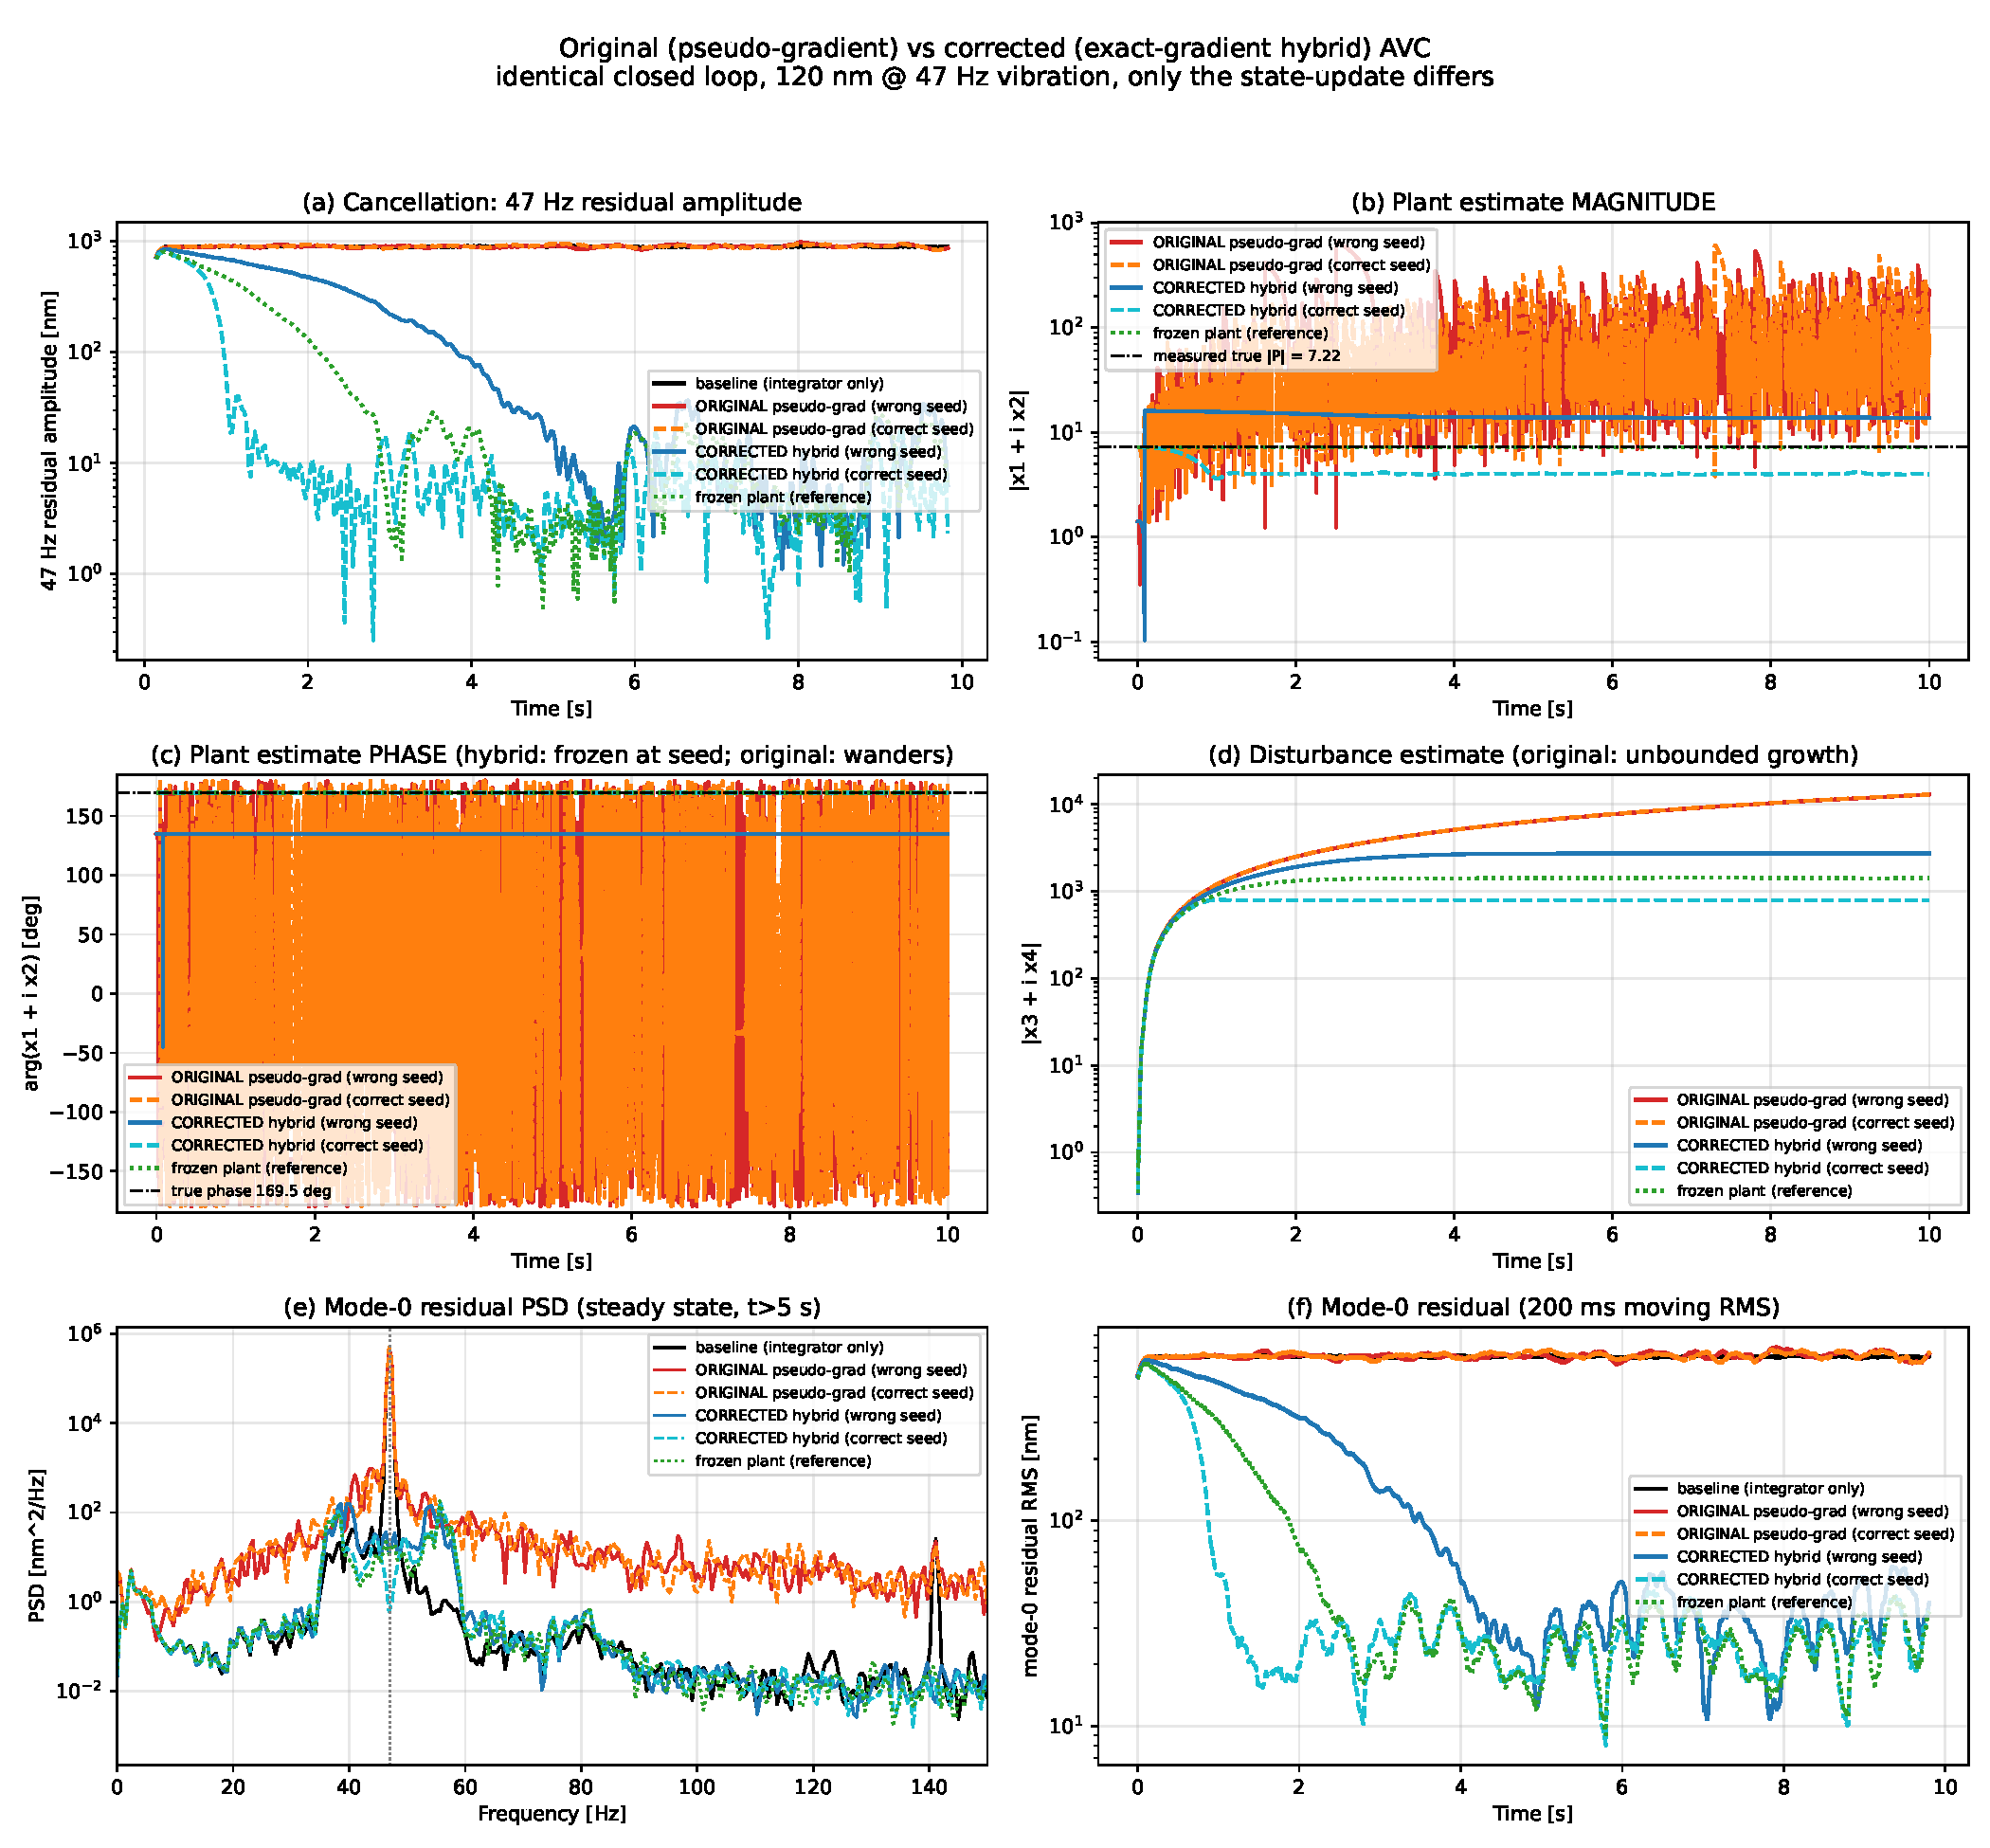
\includegraphics[width=\textwidth]{avc_gradient_comparison.pdf}
  \caption{(a) the two ORIGINAL traces remain on the baseline while the
  hybrid and the frozen reference fall by 2--3 decades; (b),(c) the
  original plant estimate wanders over three decades in magnitude and the
  full $\pm180^\circ$ in phase---violating \eqref{eq:phasemargin}---whereas
  the hybrid settles and holds its seed phase exactly, as
  \eqref{eq:g12} requires; (d) the original disturbance estimate grows
  without bound while the hybrid plateaus; (e) in the steady-state PSD the
  original \emph{enlarges} the \SI{47}{Hz} peak; (f) mode-0 residual.}
  \label{fig:cmp}
\end{figure}

The measurements match the theory point by point: the original update
violates the phase margin and fails regardless of initialisation; the
hybrid preserves it by construction and converges from either seed; the
plant phase in the hybrid runs is numerically constant, as
\eqref{eq:g12} predicts; and the wrong-seed run converges because its
$34.5^\circ$ error is inside the $90^\circ$ margin.

\section{Conclusion}

The exact gradient of the AVC cost is not a usable control law: with the
published regularisation it is identically zero, because the equation-error
cost does not depend on the parameters being optimised. Restoring it in
full removes the drive on the disturbance quadratures, whose estimate then
stays at zero and cancels nothing. The pseudo-gradient, though not a
gradient of the stated cost, is integral action on the physical residual
and converges to exact tone cancellation under a $90^\circ$ phase-margin
condition on the plant estimate. Retaining it on the disturbance while
applying the exact---and provably radial, hence margin-preserving---gradient
to the plant yields an update that cancels a \SI{47}{Hz} vibration by
$48$--$59$\,dB where the published update cancels nothing.

\paragraph{Reproducibility.}
\texttt{avc\_chainrule\_check.py} (Jacobian and Eq.~\eqref{eq:g34} against
finite differences), \texttt{params\_scao\_avc\_full\_demo.yml} (update
variant selected by \texttt{adapt\_plant} and \texttt{exact\_gradient}),
\texttt{params\_scao\_vibration\_baseline.yml},
\texttt{params\_measure\_plant.yml} (plant measurement by probe injection).
A longer companion report, \texttt{avc\_exact\_gradient.pdf}, covers the
observability analysis and the full experimental history.

\end{document}
